\documentclass{beamer}

\usepackage[utf8]{inputenc}
\usecolortheme{beaver}
\usepackage{caption}
\usepackage{subcaption}
\usepackage{mathtools}
\usepackage{todonotes}
\usepackage{amsmath}
\usepackage{bm}
\usepackage{listings}
\usepackage{ragged2e}
\usepackage{titlecaps}
\usepackage{fancyvrb}

\def\ci{\perp\!\!\!\!\!\perp}

\newtheorem{proposition}{Proposition}
\Addlcwords{for a is but and with of in as the etc on to if}

\DeclareMathOperator*{\argmax}{argmax}

\setbeamertemplate{section in toc}{\inserttocsectionnumber.~\inserttocsection}
\usetheme{Boadilla}
\makeatletter
\setbeamertemplate{footline}{%
    \leavevmode%
    \hbox{%
        \begin{beamercolorbox}[wd=.3\paperwidth,ht=2.25ex,dp=1ex,center]{author in head/foot}%
            \usebeamerfont{author in head/foot}\insertshortauthor\expandafter\beamer@ifempty\expandafter{\beamer@shortinstitute}{}{~~(\insertshortinstitute)}
        \end{beamercolorbox}%
        \begin{beamercolorbox}[wd=.55\paperwidth,ht=2.25ex,dp=1ex,center]{title in head/foot}%
            \usebeamerfont{title in head/foot}\insertshorttitle
        \end{beamercolorbox}%
        \begin{beamercolorbox}[wd=.15\paperwidth,ht=2.25ex,dp=1ex,right]{date in head/foot}%
            \usebeamerfont{date in head/foot}\insertshortdate{}\hspace*{2em}
            \insertframenumber{} / \inserttotalframenumber\hspace*{2ex} 
        \end{beamercolorbox}}%
        \vskip0pt%
    }
\makeatother

\begin{document}

\title[]{Expert-in-the-Loop Causal Discovery}
\author{Ankur Ankan}
\date{}

\maketitle

\begin{frame}{Directed Acyclic Graphs (DAGs)}
	\begin{columns}
		\begin{column}{0.55\textwidth}
		\begin{itemize}
			\item Nodes represent random variables.
			\item Edges represent causal relationships.
			\item E.g., \textbf{Education} has a direct effect on \textbf{Income}. 
			\item E.g., \textbf{Age} has indirect effect on \textbf{Income} through \textbf{Education} and \textbf{Hours Per Week}.
			\item Used for causal effect estimation.
		\end{itemize}
		\end{column}

		\begin{column}{0.45 \textwidth}
		\begin{figure}
			\centering
			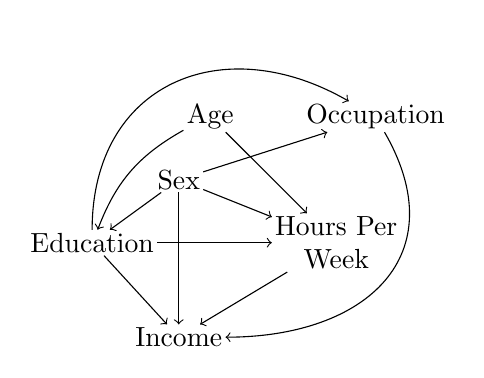
\begin{tikzpicture}[scale=1]
			\tikzstyle{every node}=[align=center, inner sep=1pt]
				\node (sex) at (-0.7, -0.8) {Sex};
				\node (age) at (-0.3, 0) {Age};
				\node (ed) at (-1.8, -1.6) {Education};
				\node (occ) at (1.8, 0) {Occupation};
				\node (hrpw) at (1.3, -1.6) {Hours Per \\ Week};
				\node (income) at (-0.7, -2.8) {Income};
			
				\draw[->]  (age) to[bend right=20] (ed);
				\draw[->]  (sex) to (ed);
				\draw[->]  (age) to (hrpw);
				\draw[->]  (ed) to (hrpw);
				\draw[->]  (sex) to (hrpw);
				\draw[->]  (ed) to (income);
				\draw[->]  (hrpw) to (income);
				\draw[->]  (occ) to[out=300, in=0, looseness=1.4] (income.east);
				\draw[->]  (sex) to (income);
				\draw[->]  (ed) to[out=90, in=150, looseness=1.3] (occ);
				\draw[->]  (sex) to (occ);	
			\end{tikzpicture}
			\caption*{\footnotesize {Example of a DAG}}
		\end{figure}
		\end{column}
	\end{columns}	
\end{frame}

\begin{frame}{Causal Discovery: Learning DAGs From Data}
	\vspace{-2em}
	\begin{figure}
		\centering
		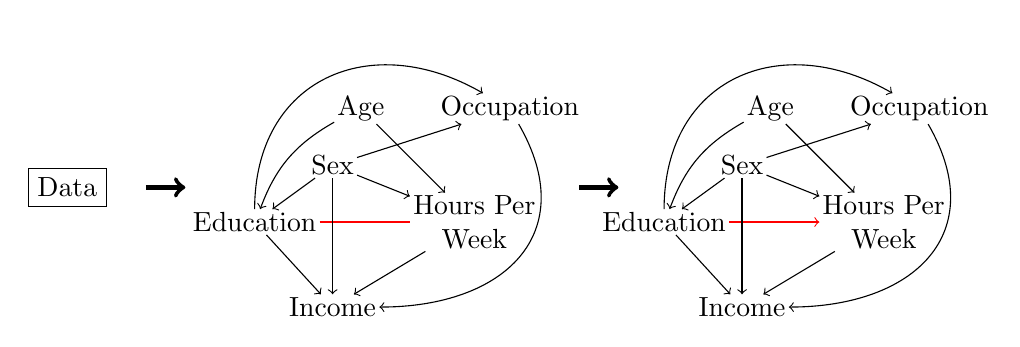
\begin{tikzpicture}
			\node[draw, rectangle] (data) at (0, 0) {Data};
			\draw[ultra thick,->] (1,0) -- (1.5,0);
			\begin{scope}[xshift=4cm, yshift=1cm, scale=0.9]
			 	\tikzstyle{every node}=[align=center, inner sep=1pt]
				\node (sex) at (-0.7, -0.8) {Sex};
				\node (age) at (-0.3, 0) {Age};
				\node (ed) at (-1.8, -1.6) {Education};
				\node (occ) at (1.8, 0) {Occupation};
				\node (hrpw) at (1.3, -1.6) {Hours Per \\ Week};
				\node (income) at (-0.7, -2.8) {Income};
			
				\draw[->]  (age) to[bend right=20] (ed);
				\draw[->]  (sex) to (ed);
				\draw[->]  (age) to (hrpw);
				\draw[-, red]  (ed) to (hrpw);
				\draw[->]  (sex) to (hrpw);
				\draw[->]  (ed) to (income);
				\draw[->]  (hrpw) to (income);
				\draw[->]  (occ) to[out=300, in=0, looseness=1.4] (income.east);
				\draw[->]  (sex) to (income);
				\draw[->]  (ed) to[out=90, in=150, looseness=1.3] (occ);
				\draw[->]  (sex) to (occ);	
			\end{scope}
			\begin{scope}[xshift=6.5cm]
				\draw[ultra thick,->] (0,0) -- (0.5,0);
			\end{scope}	
			\begin{scope}[xshift=9.2cm, yshift=1cm, scale=0.9]
				\tikzstyle{every node}=[align=center, inner sep=1pt]
				\node (sex) at (-0.7, -0.8) {Sex};
				\node (age) at (-0.3, 0) {Age};
				\node (ed) at (-1.8, -1.6) {Education};
				\node (occ) at (1.8, 0) {Occupation};
				\node (hrpw) at (1.3, -1.6) {Hours Per \\ Week};
				\node (income) at (-0.7, -2.8) {Income};
			
				\draw[->]  (age) to[bend right=20] (ed);
				\draw[->]  (sex) to (ed);
				\draw[->]  (age) to (hrpw);
				\draw[->, red]  (ed) to (hrpw);
				\draw[->]  (sex) to (hrpw);
				\draw[->]  (ed) to (income);
				\draw[->]  (hrpw) to (income);
				\draw[->]  (occ) to[out=300, in=0, looseness=1.4] (income.east);
				\draw[->]  (sex) to (income);
				\draw[->]  (ed) to[out=90, in=150, looseness=1.3] (occ);
				\draw[->]  (sex) to (occ);	
			\end{scope}
		\end{tikzpicture}
	\end{figure}

	\begin{itemize}
		\item Causal Discovery: Recover DAG from data.
		\item Many algorithms are available:
			\begin{itemize}
				\item Constraint Based: PC, FCI
				\item Score Based: Hill-Climb Search, GES
				\item Optimization Based: No Tears
			\end{itemize}
		\item Algorithms can only recover Markov Equivalence Class i.e. CPDAG.
		\item Either expert knowledge or some further assumptions can
			be make to orient the edges.
	\end{itemize}
\end{frame}

\begin{frame}{Causal Discovery in Practice}
	\begin{itemize}
		\item Adaption of causal discovery algorithms is very limited.
		\item Researchers prefer to draw models by hand based on domain knowledge.
		\item Potential reasons could be:
			\begin{itemize}
				\item Algorithms can make obvious mistakes, making it harder to trust.
				\item Hard to choose an algorithm for a given dataset because of the different assumptions.
				\item No way to evaluate algorithm performance on a given dataset.
			\end{itemize}
		\item However, some researchers do test/validate their model against data using Conditional Independence (CI) tests.
	\end{itemize}
\end{frame}

\begin{frame}{Model Testing}
	\begin{figure}
		\centering
		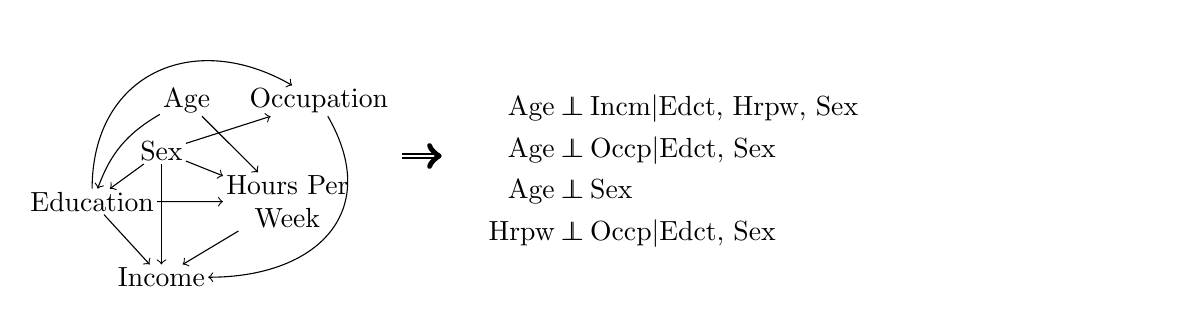
\begin{tikzpicture}
			\begin{scope}[yshift=0.7cm, scale=0.8]
			\tikzstyle{every node}=[align=center, inner sep=1pt]
				\node (sex) at (-0.7, -0.8) {Sex};
				\node (age) at (-0.3, 0) {Age};
				\node (ed) at (-1.8, -1.6) {Education};
				\node (occ) at (1.8, 0) {Occupation};
				\node (hrpw) at (1.3, -1.6) {Hours Per \\ Week};
				\node (income) at (-0.7, -2.8) {Income};
			
				\draw[->]  (age) to[bend right=20] (ed);
				\draw[->]  (sex) to (ed);
				\draw[->]  (age) to (hrpw);
				\draw[->]  (ed) to (hrpw);
				\draw[->]  (sex) to (hrpw);
				\draw[->]  (ed) to (income);
				\draw[->]  (hrpw) to (income);
				\draw[->]  (occ) to[out=300, in=0, looseness=1.4] (income.east);
				\draw[->]  (sex) to (income);
				\draw[->]  (ed) to[out=90, in=150, looseness=1.3] (occ);
				\draw[->]  (sex) to (occ);	
			\end{scope}
			\draw[thick, ->, double] (2.5,0) -- (3,0);
			\node[rectangle, align=center, inner sep=1pt] at (6, 0) {
				\begin{minipage}{\textwidth}
					\begin{equation*}
						\begin{split}
							\textnormal{Age} &\ci \textnormal{Incm} \rvert \textnormal{Edct, Hrpw, Sex} \\
							\textnormal{Age} &\ci \textnormal{Occp} \rvert \textnormal{Edct, Sex} \\
							\textnormal{Age} &\ci \textnormal{Sex} \\
							\textnormal{Hrpw} &\ci \textnormal{Occp} \rvert \textnormal{Edct, Sex} \\
						\end{split}
					\end{equation*}
				\end{minipage}
				};
		\end{tikzpicture}
	\end{figure}

	\vspace{2em}
	\begin{itemize}
		\item Each missing edge implies a Conditional Independence (CI).
		\item Statistical tests can be used to check whether they hold in data.
		\item Models can be modified based on these tests.
	\end{itemize}
\end{frame}

\begin{frame}{Model Testing: Adding Edges}
	\begin{figure}
		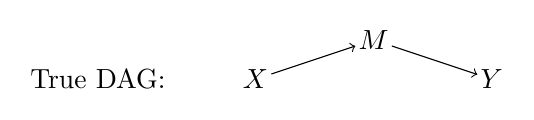
\begin{tikzpicture}[scale=1]
			\begin{scope}
				\tikzstyle{every node}=[align=center, inner sep=1pt]
					\node at (-2, 0) {True DAG:};
					\node (X) at (0, 0) {$ X $};
					\node (M) at (1.5, 0.5) {$ M $};
					\node (Y) at (3, 0) {$ Y $};
					\draw[->]  (X) to (M);
					\draw[->]  (M) to (Y);
			\end{scope}
		\end{tikzpicture}
	\end{figure}
	\vspace{1em}
	Hypothesized DAGs:
	\vspace{-1em}
	\begin{figure}
		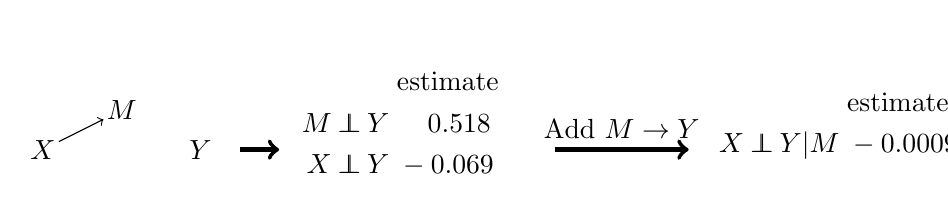
\begin{tikzpicture}
			\begin{scope}
				\tikzstyle{every node}=[align=center, inner sep=1pt]
				\node (X) at (0, 0) {$ X $};
				\node (M) at (1, 0.5) {$ M $};
				\node (Y) at (2, 0) {$ Y $};
				\draw[->]  (X) to (M);
			\end{scope}
			\begin{scope}[xshift=2cm]
				\draw[ultra thick, ->] (0.5, 0) -- (1, 0);
			\end{scope}
			\begin{scope}[xshift=4.5cm, yshift=0.5cm]
					\node at (0, 0) {
							\begin{minipage}{0.2\textwidth}
								\begin{equation*}
									\begin{split}
											& \textnormal{estimate} \\
										M \ci Y \; & \;\;\;\; 0.518 \\
										X \ci Y \; & -0.069 \\
									\end{split}
								\end{equation*}
							\end{minipage}
						};
			\end{scope}
			\draw[ultra thick, ->] (6.5, 0) -- node[above] {Add $ M \rightarrow Y $} (8.2, 0);
			\begin{scope}[xshift=9.8cm, yshift=0.5cm]
					\node at (0, 0) {
							\begin{minipage}{0.2\textwidth}
								\begin{equation*}
									\begin{split}
											& \textnormal{estimate} \\
										X \ci Y | M \; & -0.0009 \\
									\end{split}
								\end{equation*}
							\end{minipage}
						};
			\end{scope}
		\end{tikzpicture}
	\end{figure}

	\begin{figure}
		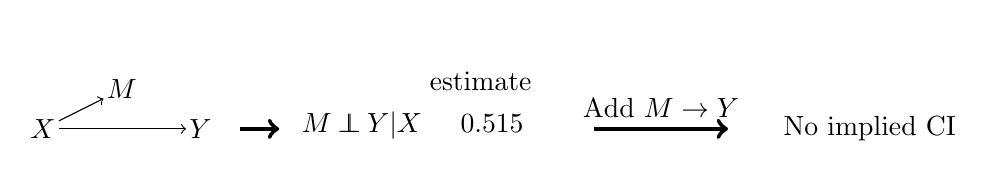
\begin{tikzpicture}
			\begin{scope}
				\tikzstyle{every node}=[align=center, inner sep=1pt]
				\node (X) at (0, 0) {$ X $};
				\node (M) at (1, 0.5) {$ M $};
				\node (Y) at (2, 0) {$ Y $};
				\draw[->]  (X) to (M);
				\draw[->]  (X) to (Y);
			\end{scope}
			\begin{scope}[xshift=2cm]
				\draw[ultra thick, ->] (0.5, 0) -- (1, 0);
			\end{scope}

			\begin{scope}[xshift=4.5cm, yshift=0.5cm]
					\node at (0, 0) {
							\begin{minipage}{0.2\textwidth}
								\begin{equation*}
									\begin{split}
											& \textnormal{estimate} \\
				 						M \ci Y \rvert X \; & \;\;\;\; 0.515 \\
									\end{split}
								\end{equation*}
							\end{minipage}
						};
			\end{scope}
			\draw[ultra thick, ->] (7, 0) -- node[above] {Add $ M \rightarrow Y $} (8.7, 0);
			\begin{scope}[xshift=10.5cm]
				\node at (0, 0) { No implied CI };
			\end{scope}
		\end{tikzpicture}
	\end{figure}
\end{frame}

\begin{frame}{Model Testing: Removing Edges}
	\begin{figure}
		\centering
		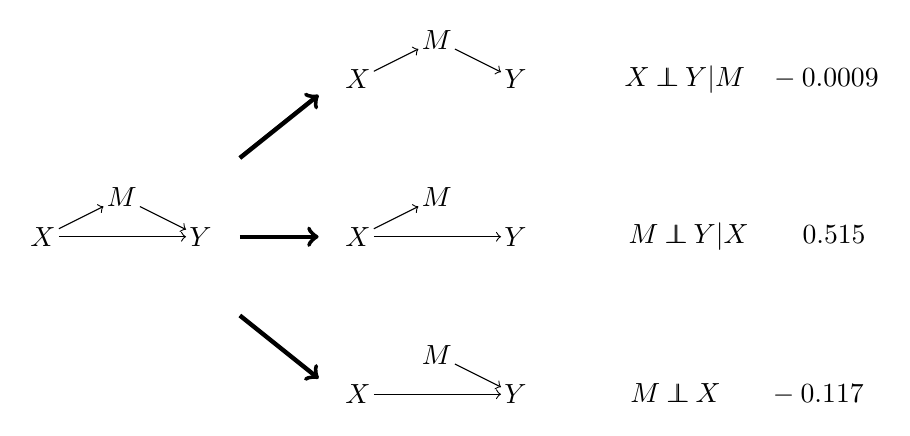
\begin{tikzpicture}
			\begin{scope}
				\tikzstyle{every node}=[align=center, inner sep=1pt]
				\node (X) at (0, 0) {$ X $};
				\node (M) at (1, 0.5) {$ M $};
				\node (Y) at (2, 0) {$ Y $};
				\draw[->] (X) to (M);
				\draw[->] (X) to (Y);
				\draw[->] (M) to (Y);
			\end{scope}

			\draw[ultra thick, ->] (2.5, 0) -- (3.5, 0);

			\begin{scope}[xshift=4cm, yshift=2cm]
				\tikzstyle{every node}=[align=center, inner sep=1pt]
				\node (X) at (0, 0) {$ X $};
				\node (M) at (1, 0.5) {$ M $};
				\node (Y) at (2, 0) {$ Y $};
				\draw[->] (X) to (M);
				\draw[->] (M) to (Y);

				\node at (5, 0) {$ X \ci Y \rvert M \;\;\; -0.0009 $};
			\end{scope}
			\draw[ultra thick, ->] (2.5, 1) -- (3.5, 1.8);
			\begin{scope}[xshift=4cm, yshift=0cm]
				\tikzstyle{every node}=[align=center, inner sep=1pt]
				\node (X) at (0, 0) {$ X $};
				\node (M) at (1, 0.5) {$ M $};
				\node (Y) at (2, 0) {$ Y $};
				\draw[->] (X) to (M);
				\draw[->] (X) to (Y);

				\node at (5, 0) { $M \ci Y \rvert X \;\;\; \;\;\;\; 0.515 $ };
			\end{scope}
			\draw[ultra thick, ->] (2.5, -1) -- (3.5, -1.8);
			\begin{scope}[xshift=4cm, yshift=-2cm]
				\tikzstyle{every node}=[align=center, inner sep=1pt]
				\node (X) at (0, 0) {$ X $};
				\node (M) at (1, 0.5) {$ M $};
				\node (Y) at (2, 0) {$ Y $};
				\draw[->] (X) to (Y);
				\draw[->] (M) to (Y);

				\node at (5, 0) { $M \ci X \;\;\;\;\;\; -0.117 $ };
			\end{scope}
		\end{tikzpicture}
	\end{figure}

\begin{itemize}
	\item Similar to estimating edge coefficients.
	\item These tests can be used to check whether the correlation present in the data is explained by the model.
\end{itemize}
\end{frame}

% \begin{frame}{Effect Sizes: Marginal Independence Tests}
% 	\centerline{Marginal Case: $ X \ci Y $}
% 
% 	\vspace{2em}
% 	
% 	\textbf{Discrete Data:} Cram\'er's V
% 		
% 	$$ V(X, Y) = \sqrt{\frac{\chi^2(X, Y) / n }{\min(k-1, r-1)}} \;\;\;\;\;\; \textnormal{where } k = \rvert X \rvert, \;\; r = \rvert Y \rvert $$
% 	\todo[inline] {Check this formula}
% 	
% 	\vspace{2em}
% 
% 	\textbf{Continuous Data:} Pearson Correlation Coefficient
% 
% 		$$ \rho(X,Y) = \frac{\textnormal{cov}(X, Y)}{\sigma_X \sigma_Y} $$
% 		
% \end{frame}
% 
% \begin{frame}{Effect Sizes: Conditional Independence Tests}
% 	\centerline{Conditional Case: $ X \ci Y \rvert \bm{Z} $}
% 
% 	\vspace{2em}
% 
% 	\textbf{Discrete Data:} Cram\'er's V
% 		\begin{itemize}
% 			\item Given a dataset $ \mathcal{D} = (X, Y, \bm{Z}) $, first stratify by conditional variable.
% 				$$ \mathcal{D} = \{ (X_{Z_1}, Y_{Z_1}, \bm{Z}_1), (X_{Z_2}, Y_{Z_2}, \bm{Z}_2), \cdots, (X_{Z_k}, Y_{Z_k}, \bm{Z}_k) \} $$
% 			\item Compute for each strata and combine them.
% 			\todo[inline]{What will it be here}
% 		\end{itemize}
% 	
% 	\vspace{2em}
% 				
% 	\textbf{Continuous Data:} Partial Correlation
% 		\begin{itemize}
% 			\item Train two estimators. $ f_x: X \sim \bm{Z} $ and $ f_y: Y \sim \bm{Z} $.
% 			\item Compute residuals: $ R_x = X - f_x(\bm{Z}) $ and $ R_y = Y - f_y(\bm{Z}) $.
% 			\item Correlation coefficient of the residuals: $ \rho_{R_x, R_y} $
% 		\end{itemize}
% 
% \end{frame}

\begin{frame}{Effect Sizes}
	We have a bunch of effect sizes for different variable types.

	\vspace{2em}
	\begin{itemize}
		\item \textbf{Continuous Variables:} Correlation coefficient, partial correlation for conditional case.
		\item \textbf{Discrete Variables:} Cram\'er's V.
		\item \textbf{Ordinal Variables: } Polychoric correlation.
		\item \textbf{Ordinal and Continuous Variables:} Polyserial correlation.
	\end{itemize}

	\vspace{2em}

	\center{But there is nothing that works for a combination of discrete, ordinal, and continuous variables.}
\end{frame}

% \begin{frame}{Effect Sizes: Mixed Data}
% 	\begin{itemize}
% 		\item We considered cases where all variables are either discrete or continuous.
% 		\item However, no effect size is available for mixed data i.e., combination of discrete, ordinal, and continuous.
% 		\item We propose one based on canonical correlations.
% 		% \item We propose an effect size measure for mixed data based on canonical correlations.
% 		% \item In the special cases, reduces to pearson correlation or cramer's V.
% 		% \item Bounded by $ 0 $ and $ 1 $.
% 	\end{itemize}
% \end{frame}

\begin{frame}{Canonical Correlations}
	Given two sets of random variables $ \bm{U} = (u_1, u_2, \cdots, u_k) $ and $ \bm{V} = (v_1, v_2, \cdots, v_r) $, canonical correlation is 
	defined as:
	\begin{equation*}
		\begin{split}
			\phi(\bm{U}, \bm{V}) &= \textnormal{cor}(a^T \bm{U}, b^T \bm{V}) \;\;\;\;\;\;\; \textnormal{where } a, b = \argmax_{(a, b)} \textnormal{cor}(a^T \bm{U}, b^T \bm{V}) \\
		\end{split}
	\end{equation*}
	\begin{itemize}
		\item Generalizes correlation coefficient to multi-dimensional variables.
		\item Finds linear combinations such that correlation is maximized.
		\item $ \rvert \phi(\bm{U}, \bm{V}) \rvert = min(k, r) $
		\item Multiple effect sizes:
			\begin{itemize}
				\item Wilks' Lambda: $ \Lambda = \prod (1 - \phi_i^2) $
				\item Roy's Largest Root: $ \theta = \phi_{\max}^2 $
				\item Pillai's Trace: $ \tau = \sum \phi_i^2 $
			\end{itemize}
		\item We use Pillai's trace.
	\end{itemize}
\end{frame}

\begin{frame}{Effect Sizes: Mixed Data}
	We want to compute the effect size for $ X \ci Y \rvert \bm{Z} $.
	
	\vspace{1em}

	\begin{itemize}
		\item If either $ X $ or $ Y $ are discrete, dummy encode them.
			$$ \textnorma{Country: } \begin{bmatrix} DE \\
					   NL \\
				           UK \\
				           NL \\
					   \cdots
					   \end{bmatrix} \implies \begin{bmatrix} 1 & 0 & 0 \\
				   						  0 & 1 & 0 \\
									          0 & 0 & 0 \\
									          0 & 1 & 0 \\
										    & \cdots &
									  \end{bmatrix}$$
		\item If $ \bm{Z} = \emptyset $, compute $ \tau(X, Y) $.
	\end{itemize}
\end{frame}

\begin{frame}{Effect Sizes: Mixed Data}
	Computing residuals:
	\begin{itemize}
		\item If $ \bm{Z} \ne \emptyset $, train two estimators $ f_x: X \sim \bm{Z} $ and $ f_y: Y \sim \bm{Z} $.
		\item Compute the residuals, $ R_x = f_x(\bm{Z}) $, and $ R_y = f_y(\bm{Z}) $.
		\item Computing residuals is not straightforward in this case.
			\begin{itemize}
				\item If continuous, difference between true and predicted.
				\item If ordinal, Li-Sheperd residuals.
				\item If categorical, treat each column as binary.
			\end{itemize}
		\item Compute $ \tau(R_x, R_y) $.
	\end{itemize}

	\footnotetext[1]{ Ankan, Ankur, and Johannes Textor. "A simple unified approach to testing high-dimensional conditional independences for categorical and ordinal data." }
\end{frame}

\begin{frame}{Human-in-the-loop Structure Learning}
	\begin{itemize}
		\item We have an effect size for mixed data.
		\item Using this effect size we built a web-based tool to assist in constructing/modifying DAGs.
		\item Given a dataset, the tool shows all unexplained correlations between variables.
		\item It also shows when certain edges do not add any extra explanation between variables.
	\end{itemize}
\end{frame}

\begin{frame}
	\center \huge DEMO
\end{frame}

\begin{frame}{Empirical Analysis: Simulate Expert}

	\begin{figure}
		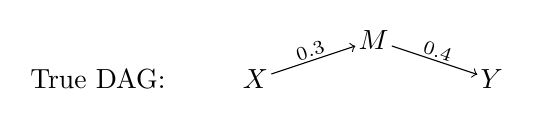
\begin{tikzpicture}[scale=1]
			\tikzstyle{every node}=[align=center, inner sep=1pt]
				\node (text) at (-2, 0) {True DAG:};
				\node (X) at (0, 0) {$ X $};
				\node (M) at (1.5, 0.5) {$ M $};
				\node (Y) at (3, 0) {$ Y $};
				\draw[->]  (X) -- node[midway, sloped, above] {\scriptsize $ 0.3 $} (M);
				\draw[->]  (M) -- node[midway, sloped, above] {\scriptsize $ 0.4 $} (Y);
		\end{tikzpicture}
	\end{figure}
	
	\vspace{2em}

	\begin{figure}
		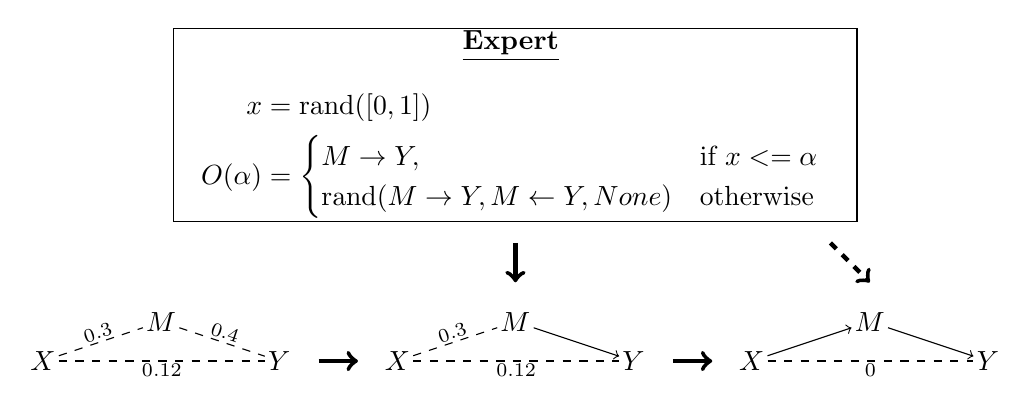
\begin{tikzpicture}
				\begin{scope}
					\tikzstyle{every node}=[align=center, inner sep=1pt]
					\node (X) at (0, 0) {$ X $};
					\node (M) at (1.5, 0.5) {$ M $};
					\node (Y) at (3, 0) {$ Y $};
					\draw[dashed]  (X) -- node[midway, sloped, above] {\scriptsize $ 0.3 $} (M);
					\draw[dashed]  (M) -- node[midway, sloped, above] {\scriptsize $ 0.4 $} (Y);
					\draw[dashed]  (X) -- node[midway, sloped, below] {\scriptsize $ 0.12 $} (Y);
				\end{scope}
				\begin{scope}[xshift=3cm]
					\draw[->, ultra thick] (0.5, 0) -- (1, 0);
				\end{scope}
				\begin{scope}[xshift=6cm, yshift=3cm]
					\node[rectangle, draw, align=center, inner sep=1pt] at (0, 0) {
							\begin{minipage}{0.7\textwidth}
								\center{\underline{\textbf{Expert}}}
								\begin{equation*}
								\begin{split}
									x &= \textnormal{rand}([0, 1]) \\
									O(\alpha) &= \begin{cases} 
										M \rightarrow Y, & \textnormal{if  } x <= \alpha \\
										\textnormal{rand}(M \rightarrow Y, M \leftarrow Y, None) & \textnormal{otherwise} \\
										     \end{cases} \\
								\end{split}
								\end{equation*}
							\end{minipage}
					};
				\end{scope}
				\begin{scope}[xshift=6cm, yshift=1cm]
					\draw[->, ultra thick] (0, 0.5) -- (0, 0);
				\end{scope}
				\begin{scope}[xshift=4.5cm]
					\tikzstyle{every node}=[align=center, inner sep=1pt]
					\node (X) at (0, 0) {$ X $};
					\node (M) at (1.5, 0.5) {$ M $};
					\node (Y) at (3, 0) {$ Y $};
					\draw[dashed]  (X) -- node[midway, sloped, above] {\scriptsize $ 0.3 $} (M);
					\draw[->]  (M) -- (Y);
					\draw[dashed]  (X) -- node[midway, sloped, below] {\scriptsize $ 0.12 $} (Y);
				\end{scope}
				\begin{scope}[xshift=7.5cm]
					\draw[->, ultra thick] (0.5, 0) -- (1, 0);
				\end{scope}
				\begin{scope}[xshift=10cm, yshift=1cm]
					\draw[dashed, ->, ultra thick] (0, 0.5) -- (0.5, 0);
				\end{scope}
				\begin{scope}[xshift=9cm]
					\tikzstyle{every node}=[align=center, inner sep=1pt]
					\node (X) at (0, 0) {$ X $};
					\node (M) at (1.5, 0.5) {$ M $};
					\node (Y) at (3, 0) {$ Y $};
					\draw[->]  (X) -- (M);
					\draw[->]  (M) -- (Y);
					\draw[dashed]  (X) -- node[midway, sloped, below] {\scriptsize $ 0 $} (Y);
				\end{scope}
		\end{tikzpicture}
	\end{figure}

	% To compare how well this approach works compared to the algorithms.

	% But need to simulate an expert/human:
	% \begin{itemize}
	% 	\item Take a greedy approach and choose the variables with the highest effect between them such that it does not create a cycle.
	% 	\item Use an oracle with a given accuracy to determine the direction of the edge.
	% 	\item After each edge addition the effects are recomputed.
	% 	\item A pruning step is done to check if adding an edge removes some of the effects.
	% \end{itemize}
\end{frame}

\begin{frame}{Empirical Analysis: Simulate Expert}
	\begin{figure}
		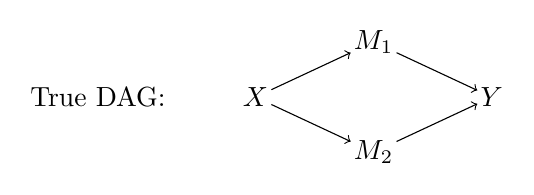
\begin{tikzpicture}[scale=1]
			\tikzstyle{every node}=[align=center, inner sep=1pt]
				\node (text) at (-2, 0) {True DAG:};
				\node (X) at (0, 0) {$ X $};
				\node (M1) at (1.5, 0.7) {$ M_1 $};
				\node (M2) at (1.5, -0.7) {$ M_2 $};
				\node (Y) at (3, 0) {$ Y $};
				\draw[->]  (X) -- (M1);
				\draw[->]  (X) -- (M2);
				\draw[->]  (M1) -- (Y);
				\draw[->]  (M2) -- (Y);
		\end{tikzpicture}
	\end{figure}

	\vspace{2em}
	\begin{figure}
	\centering
	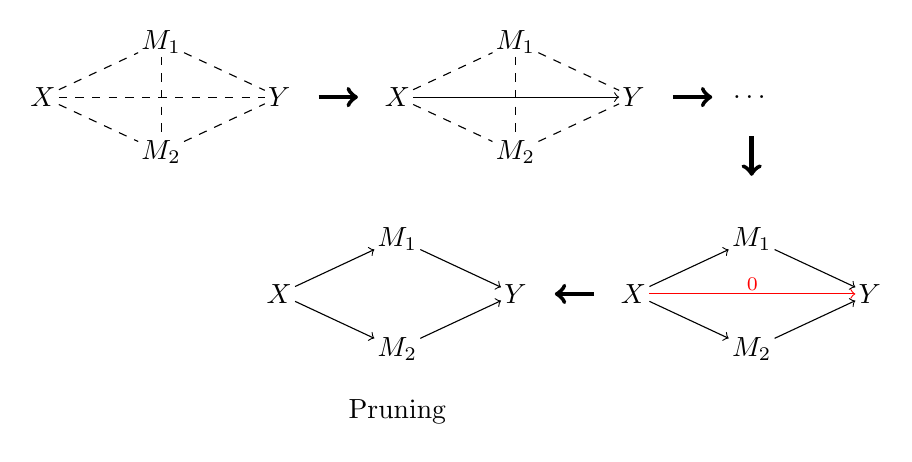
\begin{tikzpicture}
		\begin{scope}
			\tikzstyle{every node}=[align=center, inner sep=1pt]
			\node (X) at (0, 0) {$ X $};
			\node (M1) at (1.5, 0.7) {$ M_1 $};
			\node (M2) at (1.5, -0.7) {$ M_2 $};
			\node (Y) at (3, 0) {$ Y $};

			\draw[dashed]  (X) -- (M1);
			\draw[dashed]  (X) -- (M2);
			\draw[dashed]  (M1) -- (Y);
			\draw[dashed]  (M2) -- (Y);
			\draw[dashed]  (M1) -- (M2);
			\draw[dashed]  (X) -- (Y);
		\end{scope}
		\begin{scope}[xshift=3cm]
			\draw[->, ultra thick] (0.5, 0) -- (1, 0);
		\end{scope}
		\begin{scope}[xshift=4.5cm]
			\tikzstyle{every node}=[align=center, inner sep=1pt]
			\node (X) at (0, 0) {$ X $};
			\node (M1) at (1.5, 0.7) {$ M_1 $};
			\node (M2) at (1.5, -0.7) {$ M_2 $};
			\node (Y) at (3, 0) {$ Y $};

			\draw[dashed]  (X) -- (M1);
			\draw[dashed]  (X) -- (M2);
			\draw[dashed]  (M1) -- (Y);
			\draw[dashed]  (M2) -- (Y);
			\draw[dashed] (M1) -- (M2);
			\draw[->]  (X) -- (Y);
		\end{scope}
		\begin{scope}[xshift=7.5cm]
			\draw[->, ultra thick] (0.5, 0) -- (1, 0);
		\end{scope}
		\begin{scope}[xshift=9cm]
			\node at (0, 0) {$ \dots $};	
		\end{scope}
		\begin{scope}[xshift=9cm]
			\draw[->, ultra thick] (0, -0.5) -- (0, -1);
		\end{scope}
		\begin{scope}[xshift=7.5cm, yshift=-2.5cm]
			\tikzstyle{every node}=[align=center, inner sep=1pt]
			\node (X) at (0, 0) {$ X $};
			\node (M1) at (1.5, 0.7) {$ M_1 $};
			\node (M2) at (1.5, -0.7) {$ M_2 $};
			\node (Y) at (3, 0) {$ Y $};

			\draw[->]  (X) -- (M1);
			\draw[->]  (X) -- (M2);
			\draw[->]  (M1) -- (Y);
			\draw[->]  (M2) -- (Y);
			\draw[->, red]  (X) -- node[sloped, above] {\scriptsize $ 0 $} (Y);
		\end{scope}
		\begin{scope}[xshift=6.5cm, yshift=-2.5cm]
			\draw[->, ultra thick] (0.5, 0) -- (0, 0);
		\end{scope}
		\begin{scope}[xshift=3cm, yshift=-2.5cm]
			\tikzstyle{every node}=[align=center, inner sep=1pt]
			\node (X) at (0, 0) {$ X $};
			\node (M1) at (1.5, 0.7) {$ M_1 $};
			\node (M2) at (1.5, -0.7) {$ M_2 $};
			\node (Y) at (3, 0) {$ Y $};

			\draw[->]  (X) -- (M1);
			\draw[->]  (X) -- (M2);
			\draw[->]  (M1) -- (Y);
			\draw[->]  (M2) -- (Y);
		\end{scope}
		\begin{scope}[xshift=4.5cm, yshift=-4cm]
			\node at (0, 0) {Pruning};
		\end{scope}
	\end{tikzpicture}
	\caption*{Pruning Example}
	\end{figure}
\end{frame}

\begin{frame}{Empirical Analysis: Setup}
	\begin{figure}
		\centering
		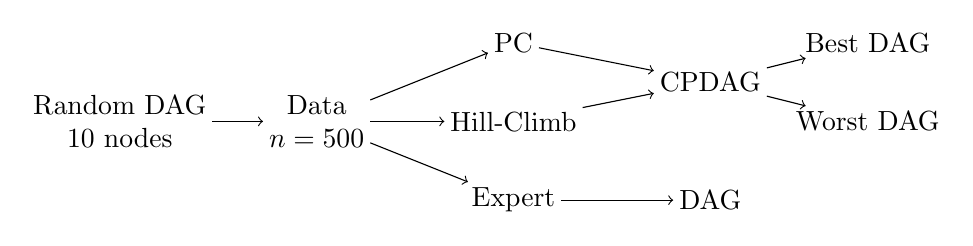
\begin{tikzpicture}
			\tikzstyle{every node}=[align=center, inner sep=2pt]
			\node (dag) at (0, 0) {Random DAG \\ $ 10 $ nodes};
			\node (data) at (2.5, 0) {Data \\ $ n=500 $};
			\node (pc) at (5, 1) {PC};
			\node (hc) at (5, 0) {Hill-Climb};
			\node (expert) at (5, -1) {Expert};
			\node (cpdag) at ( 7.5, 0.5) {CPDAG};
			\node (dag_l) at (7.5, -1) {DAG};
			\node (best_dag) at ( 9.5, 1 ) {Best DAG};
			\node (worst_dag) at ( 9.5, 0 ) {Worst DAG};

			\draw[->] (dag) -- (data);
			\draw[->] (data) -- (pc);
			\draw[->] (data) -- (hc);
			\draw[->] (data) -- (expert);
			\draw[->] (pc) -- (cpdag);
			\draw[->] (hc) -- (cpdag);
			\draw[->] (expert) -- (dag_l);
			\draw[->] (cpdag) -- (best_dag);
			\draw[->] (cpdag) -- (worst_dag);

		\end{tikzpicture}
	\end{figure}
	\vspace{2em}
	\begin{itemize}
		\item Linear mixed data is simulated.
		\item PC uses likelihood-ratio based MXM test.
		\item Hill-Climb Search uses BIC Score.
		\item The final DAGs are compared on Structural Hamming Distance (SHD) and Structural Intervention Distance (SID).
	\end{itemize}
\end{frame}


\begin{frame}
	\begin{figure}
		\centering
		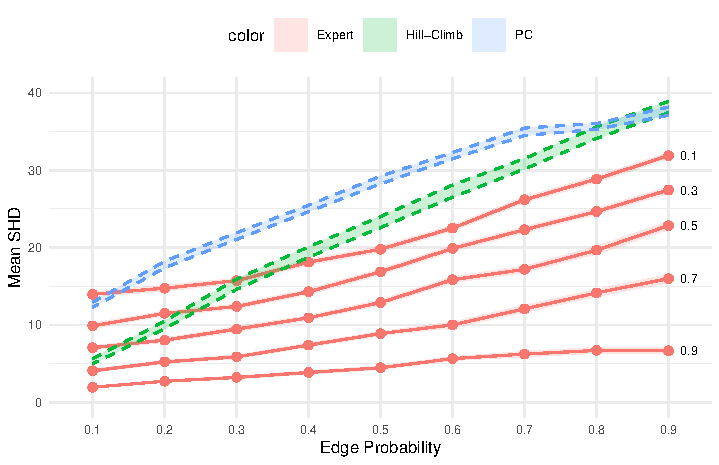
\includegraphics[scale=1]{../../2024-human-sl/code/plots/shd_ribbon.pdf}
	\end{figure}
\end{frame}

\begin{frame}
	\begin{figure}
		\centering
		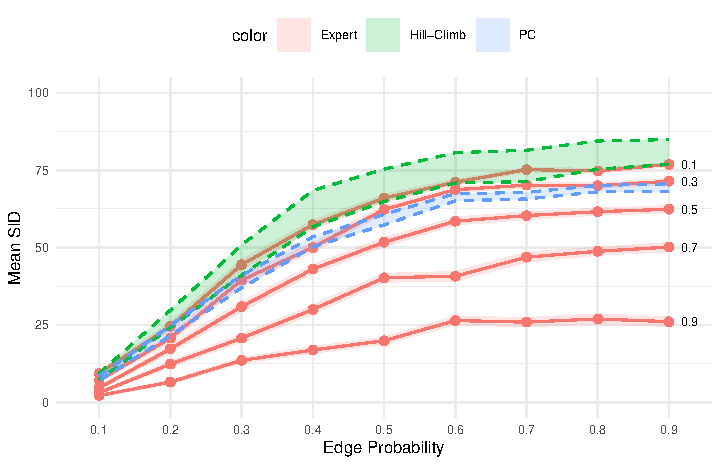
\includegraphics[scale=1]{../../2024-human-sl/code/plots/sid_ribbon.pdf}
	\end{figure}
\end{frame}

\begin{frame}{LLMs as Experts}
	\begin{itemize}
		\item Bunch of recent work in using LLMs for causal discovery.
			\begin{itemize}
				\item For determining pairwise relationships.
				\item Prompts with data.
			\end{itemize}
		\item Can we use an LLMs as experts by providing it context around variables?
	\end{itemize}
\end{frame}

\begin{frame}{Conclusion}
	\begin{itemize}
		\item We propose a generalized effect size measure for mixed data.
		\item As DAGs are predominantly drawn manually, we built a web-based tool to aid in the process.
		\item Greedy approach has a comparable performance when the expert gets $ 1 $ in $ 3 $ edge directions correctly.
		\item Implementing some back-tracking logic in expert simulation might perform better.
		\item Future work: Can LLMs be used as experts?
	\end{itemize}
\end{frame}

\end{document}
